% Лабораторная работа 3, часть 1 — презентация в Beamer
% Компилировать LuaLaTeX.
% Раздаточный материал: замените первую строку на
%   \documentclass[handout]{beamer}
\documentclass{beamer}

% --- шрифты и язык ---
\usepackage{fontspec}
\defaultfontfeatures{Renderer=Basic, Ligatures=TeX}
\newfontfamily\cyrillicfonttt{CMU Typewriter Text}
\newfontfamily\cyrillicfont{CMU Sans Serif}
\newfontfamily\cyrillicfontsf{CMU Sans Serif}
\setmainfont{CMU Sans Serif}
\setsansfont{CMU Sans Serif}
\setmonofont{CMU Typewriter Text}

\usepackage{polyglossia}
\setdefaultlanguage{russian}
\setotherlanguages{english}

% --- пакеты ---
\usepackage{graphicx}
\usepackage{listings}
\usepackage{tikz}
\usetikzlibrary{positioning, arrows.meta}

% --- тема (шаг 5) ---
\usetheme{Madrid}
\usecolortheme{default}
\setbeamertemplate{navigation symbols}{}

% --- раздаточный материал: 4 слайда на листе A4 (шаг 5) ---
\mode<handout>{
  \usepackage{pgfpages}
  \pgfpagesuselayout{4 on 1}[a4paper, border shrink=5mm, landscape]
}

% --- оформление листингов (шаг 3) ---
\lstset{
  language=Python,
  basicstyle=\ttfamily\footnotesize,
  keywordstyle=\color{blue}\bfseries,
  stringstyle=\color{orange!80!black},
  commentstyle=\color{gray}\itshape,
  frame=single,
  showstringspaces=false,
  columns=fullflexible
}

% --- титульные данные (шаг 1) ---
\title[REST API курсов ЦБ~РФ]{Асинхронный REST API курсов валют ЦБ~РФ}
\subtitle{FastAPI + SQLAlchemy}
\author[Фролов А.\,А.]{Фролов А.\,А., ИВТ-2.3}
\institute[РГПУ]{РГПУ им.~А.\,И.~Герцена}
\date{\today}

\begin{document}

% ---------- Шаг 1: титульный слайд ----------
\frame{\titlepage}

\begin{frame}
  \frametitle{Содержание}
  \tableofcontents
\end{frame}

% ============================================
\section{Задача}

% ---------- Шаг 2: списки ----------
\begin{frame}
  \frametitle{Цель и задачи}
  \textbf{Цель:} сервис, который хранит курсы валют ЦБ~РФ
  и позволяет пользователям подписываться на нужные валюты.

  \medskip
  \textbf{Задачи:}
  \begin{enumerate}
    \item Спроектировать базу данных
    \item Реализовать CRUD для пользователей
    \item Загружать курсы валют из API Банка России
    \item Реализовать подписки на валюты
  \end{enumerate}
\end{frame}

% ---------- Шаг 2: колонки ----------
\begin{frame}
  \frametitle{Стек технологий}
  \begin{columns}[T]
    \column{0.5\textwidth}
    \begin{itemize}
      \item Python
      \item FastAPI
      \item SQLAlchemy (async)
      \item Pydantic
      \item SQLite
    \end{itemize}

    \column{0.5\textwidth}
    Структура проекта:
    \begin{itemize}
      \item \texttt{models/}~--- таблицы БД
      \item \texttt{schemas/}~--- схемы Pydantic
      \item \texttt{routers/}~--- эндпоинты
      \item \texttt{services/}~--- бизнес-логика
      \item \texttt{db/}~--- подключение к БД
    \end{itemize}
  \end{columns}
\end{frame}

% ---------- Шаг 2: изображение ----------
\begin{frame}
  \frametitle{Документация API}
  \begin{center}
    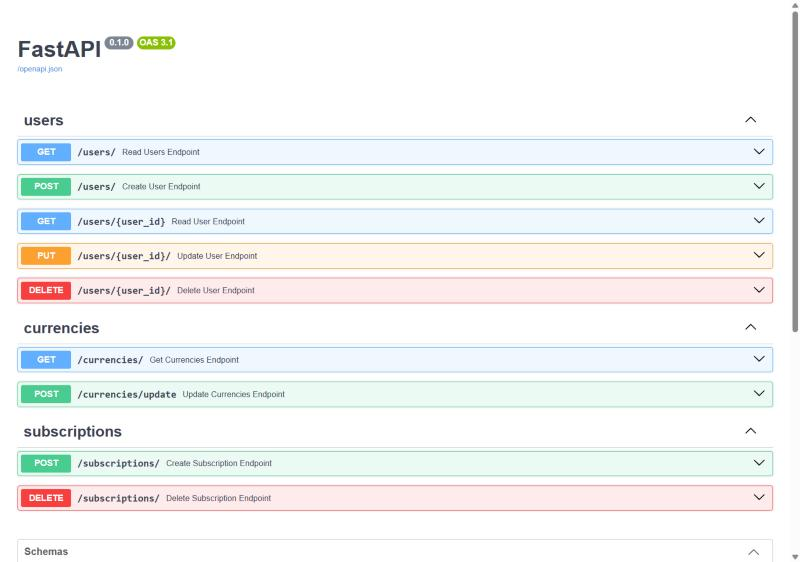
\includegraphics[width=0.72\textwidth]{swagger}

    \small Swagger UI по адресу \texttt{/docs}: все эндпоинты сервиса
  \end{center}
\end{frame}

% ---------- Шаг 2: колонки + схема ----------
\begin{frame}
  \frametitle{Архитектура}
  \begin{columns}[c]
    \column{0.55\textwidth}
    \begin{tikzpicture}[
        box/.style={draw, rounded corners, fill=blue!10,
                    minimum width=2.8cm, minimum height=0.7cm, font=\small},
        >={Stealth}, node distance=0.45cm]
      \node[box] (client) {Клиент};
      \node[box, below=of client] (routers) {routers};
      \node[box, below=of routers] (services) {services};
      \node[box, below=of services] (db) {SQLite};
      \node[box, right=0.6cm of services, fill=orange!15, minimum width=1.8cm] (cbr) {ЦБ~РФ};
      \draw[->] (client) -- (routers);
      \draw[->] (routers) -- (services);
      \draw[->] (services) -- node[right, font=\scriptsize] {SQLAlchemy} (db);
      \draw[->] (services) -- (cbr);
    \end{tikzpicture}

    \column{0.45\textwidth}
    \begin{itemize}
      \item Запрос проходит через роутер
      \item Логика вынесена в сервисы
      \item Данные хранятся в SQLite
      \item Курсы загружаются из API ЦБ~РФ
    \end{itemize}
  \end{columns}
\end{frame}

% ============================================
\section{Реализация}

% ---------- Шаг 3: блоки ----------
\begin{frame}
  \frametitle{База данных}
  \begin{block}{Таблицы}
    \textbf{User}: id, username, email, created\_at\\
    \textbf{Currency}: id, code, name, value\\
    \textbf{Subscription}: id, user\_id, currency\_id
  \end{block}

  \begin{exampleblock}{Связи}
    Один пользователь~--- много подписок; одна валюта~--- много подписок.
  \end{exampleblock}

  \begin{alertblock}{Важно}
    Все операции с БД асинхронные (\texttt{async}/\texttt{await}).
  \end{alertblock}
\end{frame}

% ---------- Шаг 3: код (listings) ----------
\begin{frame}[fragile]
  \frametitle{Пример эндпоинта}
\begin{lstlisting}
@router.get("/currencies/")
async def get_currencies(db: AsyncSession = Depends(get_db)):
    result = await db.execute(select(Currency))
    return result.scalars().all()
\end{lstlisting}
\end{frame}

% ---------- Шаг 3: код (verbatim) и гиперссылки ----------
\begin{frame}[fragile]
  \frametitle{Запуск и ссылки}
  Запуск сервера:
\begin{verbatim}
pip install -r requirements.txt
uvicorn app:app --reload
\end{verbatim}

  Ссылки:
  \begin{itemize}
    \item Репозиторий: \href{https://github.com/bluv4nul/cbrrf-rest-api}{\texttt{github.com/bluv4nul/cbrrf-rest-api}}
    \item \href{https://fastapi.tiangolo.com/}{Документация FastAPI}
    \item \href{https://www.cbr.ru/development/SXML/}{Сервисы данных Банка России}
  \end{itemize}
\end{frame}

% ============================================
\section{Итоги}

% ---------- Шаг 4: наложения ----------
\begin{frame}
  \frametitle{Эндпоинты API}
  \begin{itemize}
    \item<1-> \texttt{/users/}~--- создание, просмотр, изменение, удаление
    \item<2-> \texttt{/currencies/}~--- курсы и синхронизация с ЦБ~РФ
    \item<3-> \texttt{/subscriptions/}~--- оформление и отмена подписки
  \end{itemize}

  \onslide<4->{
    \begin{block}{Итог}
      Все задачи выполнены, API работает асинхронно.
    \end{block}
  }
\end{frame}

\begin{frame}
  \frametitle{Выводы}
  \begin{itemize}[<+->]
    \item Освоен асинхронный стек FastAPI + SQLAlchemy
    \item Реализована интеграция со внешним API
    \item Код разделён на слои: модели, схемы, роутеры, сервисы
    \item \alert{Дальше:} тесты и развёртывание в Docker
  \end{itemize}
\end{frame}

% ---------- Шаг 5: слайд только для раздаточного материала ----------
\begin{frame}<beamer:0>
  \frametitle{Для раздаточного материала}
  Этот слайд виден только в режиме \texttt{handout}.

  Исходный код: \texttt{github.com/bluv4nul/cbrrf-rest-api}
\end{frame}

\begin{frame}
  \begin{center}
    \Huge Спасибо за внимание!
  \end{center}
\end{frame}

\end{document}
